\subsection{Motzkin Number}{\label{pp:motzkinnumber}}
Consider a grid with $n$ horizontal lines and $n$ vertical lines. A Motzkin Number is defined as the number of paths from bottom-left corner of the grid to the bottom-right corner which always stays on or above $x-$axis by walking horizontally fowards \emph{or diagonally upwards or diagonally downwards}; so, the person is constrained to move only in positive $x$ and along $y=x$ or $y=-x$ ($y$ direction can be negative).
\begin{figure}[H]
	\centering
	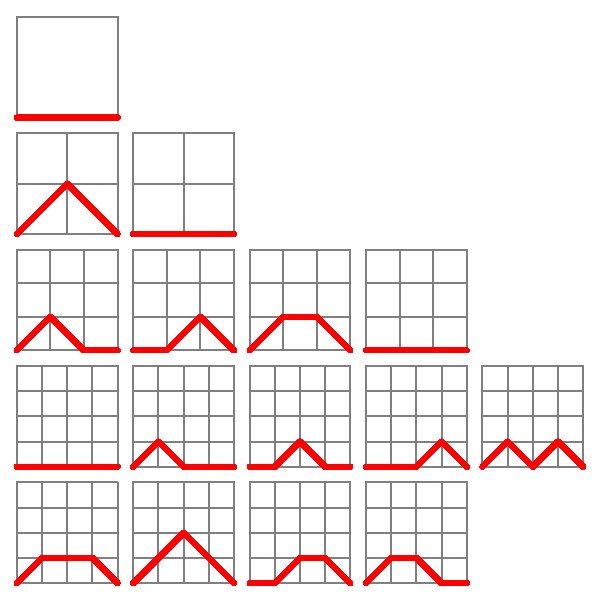
\includegraphics[width = 0.32\linewidth]{Motzkin Number.pdf}
	\caption{Example walks for case $n=1\ (\#1),\ n=2\ (\#2),\ n=3\ (\#4),\ n=4\ (\#9)$ (\href{https://mathworld.wolfram.com/MotzkinNumber.html}{Image Source})}
	\label{fig:motzkinnumber}
\end{figure}
\vspace{-1em}
\textbf{Problem Statement:}\\
Find the \emph{Motzkin Number} for a given $n$ (for all test cases).
\begin{testcasesFunction}
	{$t$ \hfill(number of test cases, an integer)\\
	$n_1\ n_2\ \ldots n_t$ \hfill($t$ space seperated integers for each testcase)}
	{Number of Motzkin Numbers for $n_i$  \hfill(each test case on a newline)}
	{$1 \leq n_i \leq 20$}
	{\texttt{int motzkin\_number(int n)} -- returns the number of possible walks for $n$.}
	{10\\1 2 3 4 5 8 11 14 17 20}
	{1\\2\\4\\9\\21\\323\\5798\\113634\\2356779\\50852019}
	{https://github.com/paramrathour/CS-101/tree/main/Starter Codes/Motzkin Number.cpp}
\end{testcasesFunction}